\documentclass[10pt,leqno]{article}

\usepackage[%
  tmargin=1.2in,bmargin=1.2in,%
  lmargin=1.8in,rmargin=1.8in,%
]{geometry}
\usepackage{fancyhdr}
\usepackage{titlesec}
\usepackage{appendix}
\usepackage{microtype}
\usepackage[hyphens]{url}
\usepackage{enumitem}
\usepackage{xspace}
\usepackage{etoolbox}
\usepackage{ifthen}
\usepackage{tikz}
\usepackage{tikz-cd}

\usepackage{amsmath}
\definecolor{darkred}{rgb}{0.5,0.0,0.0}
\usepackage[%
  colorlinks,%
  linkcolor=darkred,%
  citecolor=darkred,%
  urlcolor=darkred,%
]{hyperref}
\usepackage{amsthm,amssymb}
% \usepackage[lining,semibold]{libertine}
% \usepackage{textcomp,stmaryrd}
% \usepackage[libertine,cmintegrals,bigdelims]{newtxmath}
% \useosf
% \usepackage[%
%   cal=boondox, calscaled=0.97,%
%   bb=boondox, bbscaled=0.98,%
% ]{mathalfa}
\usepackage{cleveref}

\frenchspacing
\urlstyle{rm}

\AtBeginDocument{%
  \setlength{\abovedisplayskip}{1.5ex plus 0.3ex minus 0.3ex}%
  \setlength{\abovedisplayshortskip}{1.0ex plus 0.3ex minus 0.3ex}%
  \setlength{\belowdisplayskip}{1.5ex plus 0.3ex minus 0.3ex}%
  \setlength{\belowdisplayshortskip}{1.0ex plus 0.3ex minus 0.3ex}%
}

\let\theoldbibliography\thebibliography
\renewcommand{\thebibliography}[1]{%
  \theoldbibliography{#1}%
  \setlength{\parskip}{0ex}
  \setlength{\itemsep}{0.5ex plus 0.2ex minus 0.2ex}
  \small
}

\pagestyle{fancy}
\renewcommand{\headrulewidth}{0pt}
\renewcommand{\footrulewidth}{0pt}
\fancyhf{}
\fancyfoot[C]{\small\thepage}

\renewcommand{\title}[1]{\newcommand{\thetitle}{#1}}
\renewcommand{\author}[1]{\newcommand{\theauthor}{#1}}
\renewcommand{\date}[1]{\newcommand{\thedate}{#1}}

\renewcommand{\maketitle}{%
  \begin{center}
    {\bfseries\MakeUppercase{%
      \thetitle}}\\[2.5ex]
    {\footnotesize\MakeUppercase{%
      \theauthor}}\\[2.5ex]
    \ifthenelse{\equal{\thedate}{}}{}{%
      \small%
      \setlength{\tabcolsep}{0.2em}%
      \begin{tabular}{rl}
        original: & \thedate \\
        updated: & \today
      \end{tabular}
    }
  \end{center}
  \vspace{2.5ex}
  \thispagestyle{fancy}
}

%%%%%%%%%%%%%%%%%%%%%%%%%%%%%%%%%%%%%%%%%%%%%%%%%%%%%%%%%%%%%%%%%%%%%%

\cspreto{section}{\setcounter{equation}{0}}

\titleformat{\section}{\centering\scshape}{\thesection.}{0.4em}{}
\titlespacing{\section}{0pt}{*4}{*1}
\titleformat{\subsection}{\scshape}{\thesubsection.}{0.4em}{}
\titlespacing{\subsection}{0pt}{*2.5}{*1}

% Display format for equations
\newcommand{\crefeqfmt}[1]{
  \crefformat{#1}{(##2##1##3)}
  \Crefformat{#1}{(##2##1##3)}
  \crefrangeformat{#1}{(##3##1##4--##5##2##6)}
  \Crefrangeformat{#1}{(##3##1##4--##5##2##6)}
  \crefmultiformat{#1}{(##2##1##3}{, ##2##1##3)}{, ##2##1##3}{, ##2##1##3)}
  \Crefmultiformat{#1}{(##2##1##3}{, ##2##1##3)}{, ##2##1##3}{, ##2##1##3)}
  \crefrangemultiformat{#1}{(##3##1##4--##5##2##6}{, ##3##1##4--##5##2##6)}{, ##3##1##4--##5##2##6}{, ##3##1##4--##5##2##6)}
  \Crefrangemultiformat{#1}{(##3##1##4--##5##2##6}{, ##3##1##4--##5##2##6)}{, ##3##1##4--##5##2##6}{, ##3##1##4--##5##2##6)}
}
% Display format for sections
\newcommand{\crefsecfmt}[1]{%
  \crefformat{#1}{\S##2##1##3}
  \Crefformat{#1}{\S##2##1##3}
  \crefrangeformat{#1}{\S\S##3##1##4--##5##2##6}
  \Crefrangeformat{#1}{\S\S##3##1##4--##5##2##6}
  \crefmultiformat{#1}{\S\S##2##1##3}{ and~##2##1##3}{, ##2##1##3}{ and~##2##1##3}
  \Crefmultiformat{#1}{\S\S##2##1##3}{ and~##2##1##3}{, ##2##1##3}{ and~##2##1##3}
  \crefrangemultiformat{#1}{\S\S##3##1##4--##5##2##6}{ and~##3##1##4--##5##2##6}{, ##3##1##4--##5##2##6}{ and~##3##1##4--##5##2##6}
  \Crefrangemultiformat{#1}{\S\S##3##1##4--##5##2##6}{ and~##3##1##4--##5##2##6}{, ##3##1##4--##5##2##6}{ and~##3##1##4--##5##2##6}
}
\crefeqfmt{equation}
\crefeqfmt{enumi}
\crefeqfmt{enumii}
\crefsecfmt{section}
\crefsecfmt{subsection}
\crefsecfmt{appendix}
\crefname{part}{Part}{Parts}
\crefname{chapter}{Chapter}{Chapters}
\crefname{figure}{Figure}{Figures}

\makeatletter

\newcommand{\thmnumfont}{\bfseries}
\newcommand{\thmheadfont}{\bfseries}
\newcommand{\thmnotefont}{\bfseries}
\newcommand{\thmhorizspace}{0.4em}

\def\swappedhead#1#2#3{%
  \thmnumber{\@upn{{\thmnumfont#2}}\@ifnotempty{#1}{.\hspace{0.25em}}}%
  \thmheadfont\thmname{#1}%
  \@ifnotempty{#3}{\ \thmnote{\thmnotefont(#3)}}%
}
\swapnumbers

\newtheoremstyle{block}%
  {2.0ex plus 0.2ex minus 0.1ex}% Space above
  {2.0ex plus 0.2ex minus 0.1ex}% Space below
  {} % Body font
  {} % Indent amount
  {\thmheadfont} % Theorem head font
  {.} % Punctuation after theorem head
  {\thmhorizspace} % Space after theorem head
  {} % Theorem head spec (can be left empty, meaning ‘normal’)

\renewenvironment{proof}[1][Proof]{\par
  \pushQED{\qed}%
  \normalfont%
  \topsep1ex plus 0.2ex minus 0.1ex\relax%
  \labelsep \thmhorizspace\relax%
  \trivlist
  \item[\hskip\labelsep\thmheadfont
    #1\@addpunct{.}]\ignorespaces
}{%
  \popQED\endtrivlist\@endpefalse%
}

\makeatother

\theoremstyle{block}

\newcommand{\defthm}[2]{%
  \newtheorem{#1}[equation]{#2}%
  \crefeqfmt{#1}%
  \newtheorem*{#1*}{#2}%
}

\defthm{algorithm}{Algorithm}
\defthm{conjecture}{Conjecture}
\defthm{construction}{Construction}
\defthm{convention}{Convention}
\defthm{corollary}{Corollary}
\defthm{definition}{Definition}
\defthm{definitions}{Definitions}
\defthm{example}{Example}
\defthm{examples}{Examples}
\defthm{exercise}{Exercise}
\defthm{fact}{Fact}
\defthm{intuition}{Intuition}
\defthm{lemma}{Lemma}
\defthm{notation}{Notation}
\defthm{nothing}{}
\defthm{proposition}{Proposition}
\defthm{question}{Question}
\defthm{remark}{Remark}
\defthm{remarks}{Remarks}
\defthm{situtation}{Situation}
\defthm{theorem}{Theorem}

\setlist{%
  leftmargin=2.5em, parsep=0ex, listparindent=\parindent,
  itemsep=1.0ex, topsep=1.0ex,%
}

\setlist[enumerate, 1]{%
  label=(\alph*),%
  ref=\alph*,%
  widest=d,%
}
\setlist[enumerate, 2]{%
  label=(\roman*),%
  ref=\theenumi.\roman*,%
}
\setlist[itemize, 1]{%
  label=$\vcenter{\hbox{\footnotesize$\bullet$}}$,%
}
\setlist[itemize, 2]{label=--}

%%%%%%%%%%%%%%%%%%%%%%%%%%%%%%%%%%%%%%%%%%%%%%%%%%%%%%%%%%%%%%%%%%%%%%

\makeatletter

\let\ea\expandafter

\newcount\foreachcount

\def\foreachletter#1#2#3{\foreachcount=#1
  \ea\loop\ea\ea\ea#3\@alph\foreachcount
  \advance\foreachcount by 1
  \ifnum\foreachcount<#2\repeat}

\def\foreachLetter#1#2#3{\foreachcount=#1
  \ea\loop\ea\ea\ea#3\@Alph\foreachcount
  \advance\foreachcount by 1
  \ifnum\foreachcount<#2\repeat}

% Roman: \rA is \mathrm{A}
\def\definerm#1{%
  \ea\gdef\csname r#1\endcsname{\ensuremath{\mathrm{#1}}\xspace}}
\foreachLetter{1}{27}{\definerm}
\foreachletter{1}{27}{\definerm}
% Script: \sA is \mathscr{A}
\def\definescr#1{%
  \ea\gdef\csname s#1\endcsname{\ensuremath{\mathscr{#1}}\xspace}}
\foreachLetter{1}{27}{\definescr}
% Calligraphic: \cA is \mathcal{A}
\def\definecal#1{%
  \ea\gdef\csname c#1\endcsname{\ensuremath{\mathcal{#1}}\xspace}}
\foreachLetter{1}{27}{\definecal}
% Bold: \bA is \mathbf{A}
\def\definebold#1{%
  \ea\gdef\csname b#1\endcsname{\ensuremath{\mathbf{#1}}\xspace}}
\foreachLetter{1}{27}{\definebold}
% Blackboard Bold: \lA is \mathbb{A}
\def\definebb#1{%
  \ea\gdef\csname l#1\endcsname{\ensuremath{\mathbb{#1}}\xspace}}
\foreachLetter{1}{27}{\definebb}
% Fraktur: \ka is \mathfrak{a}, \kA is \mathfrak{A}
\def\definefrak#1{%
  \ea\gdef\csname k#1\endcsname{\ensuremath{\mathfrak{#1}}\xspace}}
\foreachletter{1}{27}{\definefrak}
\foreachLetter{1}{27}{\definefrak}
% Sans serif: \iA \is \mathsf{A}
\def\definesf#1{%
  \ea\gdef\csname i#1\endcsname{\ensuremath{\mathsf{#1}}\xspace}}
\foreachletter{1}{6}{\definesf}
\foreachletter{7}{14}{\definesf}
\foreachletter{15}{27}{\definesf}
\foreachLetter{1}{27}{\definesf}
% Bar: \Abar is \overline{A}, \abar is \overline{a}
\def\definebar#1{%
  \ea\gdef\csname #1bar\endcsname{\ensuremath{\overline{#1}}\xspace}}
\foreachLetter{1}{27}{\definebar}
\foreachletter{1}{8}{\definebar} % \hbar is something else!
\foreachletter{9}{15}{\definebar} % \obar is something else!
\foreachletter{16}{27}{\definebar}
% Tilde: \Atil is \widetilde{A}, \atil is \widetilde{a}
\def\definetil#1{%
  \ea\gdef\csname #1til\endcsname{\ensuremath{\widetilde{#1}}\xspace}}
\foreachLetter{1}{27}{\definetil}
\foreachletter{1}{27}{\definetil}
% Hats: \Ahat is \widehat{A}, \ahat is \widehat{a}
\def\definehat#1{%
  \ea\gdef\csname #1hat\endcsname{\ensuremath{\widehat{#1}}\xspace}}
\foreachLetter{1}{27}{\definehat}
\foreachletter{1}{27}{\definehat}
% Checks: \Achk is \widecheck{A}, \achk is \widecheck{a}
\def\definechk#1{%
  \ea\gdef\csname #1chk\endcsname{\ensuremath{\widecheck{#1}}\xspace}}
\foreachLetter{1}{27}{\definechk}
\foreachletter{1}{27}{\definechk}
% Underline: \Aund is \underline{A}, \aund is \underline{a}
\def\defineul#1{%
  \ea\gdef\csname #1und\endcsname{\ensuremath{\underline{#1}}\xspace}}
\foreachLetter{1}{27}{\defineul}
\foreachletter{1}{27}{\defineul}

\makeatother

%%%%%%%%%%%%%%%%%%%%%%%%%%%%%%%%%%%%%%%%%%%%%%%%%%%%%%%%%%%%%%%%%%%%%%

\usetikzlibrary{calc,decorations.pathmorphing,shapes,arrows}
\tikzcdset{
  arrow style=tikz,
  diagrams={>={stealth}},
}

\newcommand{\arrlen}{1em}
\renewcommand{\to}{\mathrel{\tikz[baseline]%
    \draw[>=stealth,->](0,0.5ex)--(\arrlen,0.5ex);}}
\newcommand{\from}{\mathrel{\tikz[baseline]%
    \draw[>=stealth,<-](0,0.5ex)--(\arrlen,0.5ex);}}
\renewcommand{\mapsto}{\mathrel{\tikz[baseline]%
    \draw[>=stealth,|->](0,0.5ex)--(\arrlen,0.5ex);}}
\newcommand{\inj}{\mathrel{\tikz[baseline]%
    \draw[>=stealth,right hook->](0,0.5ex)--(\arrlen,0.5ex);}}
\newcommand{\surj}{\mathrel{\tikz[baseline]%
    \draw[>=stealth,->>](0,0.5ex)--(\arrlen,0.5ex);}}
\newcommand{\fromto}{\mathrel{%
  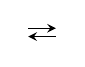
\begin{tikzpicture}[baseline]%
    \draw[>=stealth,<-](0,0.15ex)--(\arrlen,0.15ex);%
    \draw[>=stealth,->](0,0.85ex)--(\arrlen,0.85ex);%
  \end{tikzpicture}}}
\newcommand{\doubto}{\mathrel{%
  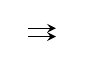
\begin{tikzpicture}[baseline]%
    \draw[>=stealth,->](0,0.15ex)--(\arrlen,0.15ex);%
    \draw[>=stealth,->](0,0.85ex)--(\arrlen,0.85ex);%
  \end{tikzpicture}}}
\newcommand{\lblto}[1]{\mathrel{%
    \begin{tikzpicture}[baseline= {( $ (current bounding box.south) + (0,-0.5ex) $ )}]
      \node[inner sep=.4ex] (a) {\,$\scriptstyle #1$\,};
      \draw[>=stealth,->] (a.south west) -- (a.south east);
    \end{tikzpicture}}}
\newcommand{\isoto}{\lblto{\sim}}

\newcommand{\simpl}[3]{
  \begin{tikzcd}[ampersand replacement=\&, column sep=small]
    #1 \&
    #2 \ar[l, shift right=0.35ex]
       \ar[l, shift left=0.35ex] \&
    #3 \ar[l, shift right=0.70ex]
       \ar[l, shift left=0.70ex]
       \ar[l] \&
    \cdots \ar[l, shift right=0.35ex]
           \ar[l, shift left=0.35ex]
           \ar[l, shift right=1.05ex]
           \ar[l, shift left=1.05ex]
  \end{tikzcd}
}
\newcommand{\cosimpl}[3]{
  \begin{tikzcd}[ampersand replacement=\&, column sep=small]
    #1 \ar[r, shift right=0.35ex]
       \ar[r, shift left=0.35ex] \&
    #2 \ar[r, shift right=0.70ex]
       \ar[r, shift left=0.70ex]
       \ar[r] \&
    #3 \ar[r, shift right=0.35ex]
       \ar[r, shift left=0.35ex]
       \ar[r, shift right=1.05ex]
       \ar[r, shift left=1.05ex] \&
    \cdots
  \end{tikzcd}
}

\newcommand{\tto}{\mathrel{\tikz[baseline]%
    \draw[>=stealth,->,double, double distance = 0.3ex](0,0.5ex)--(\arrlen,0.5ex);}}
\newcommand{\doubfrom}{\mathrel{%
  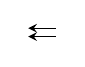
\begin{tikzpicture}[baseline]%
    \draw[>=stealth,<-](0,0.15ex)--(\arrlen,0.15ex);%
    \draw[>=stealth,<-](0,0.85ex)--(\arrlen,0.85ex);%
  \end{tikzpicture}}}
\newcommand{\tripfrom}{\mathrel{%
  
\begin{tikzpicture}[baseline]%
    \draw[>=stealth,<-](0,0.00ex)--(\arrlen,0.00ex);%
    \draw[>=stealth,<-](0,0.50ex)--(\arrlen,0.50ex);%
    \draw[>=stealth,<-](0,1.00ex)--(\arrlen,1.00ex);%
  \end{tikzpicture}}}


\renewcommand{\l}{\left}
\renewcommand{\r}{\right}
\newcommand{\f}{\frac}
\renewcommand{\o}{\overline}
\renewcommand{\u}{\underline}
\newcommand{\til}{\widetilde}
\renewcommand{\hat}{\widehat}
\newcommand{\del}{\partial}
\newcommand{\dash}{\text{-}}
\renewcommand{\c}{\colon}
\newcommand{\lc}{\,:\!}
\newcommand{\ce}{\coloneq}%{\mathrel{:=}}
\newcommand{\ec}{\eqcolon}%{\mathrel{=:}}
\newcommand{\iso}{\simeq}
\newcommand{\dual}{\vee}
\newcommand{\ldb}{\llbracket}
\newcommand{\rdb}{\rrbracket}

\newcommand{\Obj}{\operatorname{Obj}}
\newcommand{\Hom}{\operatorname{Hom}}
\newcommand{\Map}{\operatorname{Map}}
\newcommand{\Fun}{\operatorname{Fun}}
\newcommand{\Aut}{\operatorname{Aut}}
\newcommand{\Iso}{\operatorname{Iso}}
\renewcommand{\id}{\mathrm{id}}
\renewcommand{\im}{\operatorname{im}}
\newcommand{\op}{\mathrm{op}}
\newcommand{\univ}{\mathrm{univ}}
\newcommand{\colim}{\operatorname*{colim}}
\newcommand{\dlim}{\displaystyle\lim}
\newcommand{\dcolim}{\displaystyle\colim}
\newcommand{\Spec}{\operatorname{Spec}}
\newcommand{\Spf}{\operatorname{Spf}}

%%%%%%%%%%%%%%%%%%%%%%%%%%%%%%%%%%%%%%%%%%%%%%%%%%%%%%%%%%%%%%%%%%%%%%


\title{Math 216A Homework 8}
\author{Arpon Raksit}
\date{November 17, 2016}

\numberwithin{block}{section}

%%%%%%%%%%%%%%%%%%%%%%%%%%%%%%%%%%%%%%%%%%%%%%%%%%%%%%%%%%%%%%%%%%%%%%

\begin{document}
\maketitle


%%%%%%%%%%%%%%%%%%%%%%%%%%%%%%%%%%%%%%%%%%%%%%%%%%%%%%%%%%%%%%%%%%%%%%

\section{Reducing valuative criteria to DVRs}

\begin{nothing}
  \label{dvr-dom}
  Let $(\sO,\km)$ be a noetherian local domain with fraction field $K$.

  \begin{sublemma}
    \label{dvr-dom-good-gens}
    Let $\{x_1,\ldots,x_n\}$ be a set of generators for $\km$. Then there exists $i \in \{1,\ldots,n\}$ such that if we define $\sO' \ce \sO[x_1/x_i,\ldots,x_n/x_i] \subseteq K$ then the principal ideal $(x_i)$ of $\sO'$ is not the unit ideal.

    \begin{proof}
      Choose a valuation ring $(A,\km_A)$ of $K$ dominating $(\sO,\km)$ (Matsumura, Theorem 10.2), and let $v \c K^\times \to \Gamma$ be the associated valuation. Recall this means
      \[
        A = \{x \in K^\times : v(x) \ge 0\} \cup \{0\}, \quad
        \km_A = \{x \in K^\times : v(x) > 0\} \cup \{0\},
      \]
      so since $A$ dominates $\sO$ we know $v(x_1),\ldots,v(x_n) > 0$. We choose $i \in \{1,\ldots,n\}$ such that $v(x_i)$ is minimal among $v(x_1),\ldots,v(x_n)$. Then clearly $\sO' \subseteq A$. And so the intersection $\km_A \cap \sO'$ is a prime ideal, in particular is not the unit ideal. Since $x_1 \in \km_A$, the claim follows.
    \end{proof}
  \end{sublemma}

  \begin{sublemma}
    \label{dvr-dom-dim-1}
    There is a noetherian local domain $(\sO'',\km'') \subseteq K$ of dimension $1$ dominating $(\sO,\km)$.

    \begin{proof}
      Let $\{x_1,\ldots,x_n\}$ be a set of generators for $\km$. Choose $i \in \{1,\ldots,n\}$ and define $\sO'$ as in \cref{dvr-dom-good-gens}. Then $(x_i) \subseteq \sO'$ is not the unit ideal so we may choose a minimal prime ideal $\kp$ containing it. Define $(\sO'',\km'') \ce (\sO'_\kp,\kp\sO'_\kp)$. This is evidently a local domain, and is noetherian since it is a localization of $\sO'$, which is noetherian by construction since $\sO$ is. It is dimension $1$ by the hauptidealsatz. Finally, $\km'' \cap \sO$ is a prime ideal in $\sO$ evidently containing $x_1,\ldots,x_n$, and hence must be $\km$, so indeed this dominates $\sO$.
    \end{proof}
  \end{sublemma}

  \begin{subproposition}
    \label{dvr-dom-krull-akizuki}
    Let $L$ be a finitely generated field extension of $K$. Then there exists a discrete valuation ring $(R,\km_R)$ of $L$ dominating $(\sO,\km)$.

    \begin{proof}
      First observe that we may replace $(K,\sO,\km)$ with any $(K',\sO',\km')$ where $K'$ is an intermediate extension of $L/K$ and $(\sO',\km')$ is a noetherian local domain in $K'$ dominating $(\sO,\km)$. This gives us two reductions:
      \begin{itemize}
      \item If $L$ is an extension of a transcendental intermediate field $K' = K(t)$, then we may take $\sO' = \sO[t]$ and $\km'$ to be any maximal ideal containing $\km\sO'$. This reduces us to the case that $L$ is a finite extension of $K$.
      \item By \cref{dvr-dom-dim-1} we are reduced us to the case that $\sO$ is dimension $1$.
      \end{itemize}
      
      Now let $\til\sO$ be the integral closure of $\sO$ in $L$. By Krull-Akizuki (Matsumura, Corollary to Theorem 11.7), $\til\sO$ is a Dedekind domain. Thus if we take $\til\km$ to be any maximal ideal of $\til\sO$ containing $\km\til\sO$, the localization $(R,\km_R) \ce (\til\sO_{\til\km},\til\km\til\sO_{\til\km})$ will be a DVR. The intersection $\km_R \cap \sO$ is a prime ideal containing $\km$ and hence must be $\km$, so $R$ indeed dominates $\sO$.
    \end{proof}
  \end{subproposition}
\end{nothing}

%%%%%%%%%%%%%%%%%%%%%%%%%%%%%%%%%%%%%%%%%%%%%%%%%%%%%%%%%%%%%%%%%%%%%%

\begin{nothing}
  \label{valcrit}
  We now explain how in the noetherian setting we may use
  \cref{dvr-dom-krull-akizuki} to reduce the checking of valuative
  criteria to the case of discrete valuation rings.

  \begin{subproposition}
    \label{valcrit-sep}
    Let $X$ be a locally noetherian scheme. Let $f \c X \to Y$ be a map locally of finite type. Then $f$ is separated if and only if $f$ satisfies the valuative criterion for separatedness for discrete valuation rings.

    \begin{proof}
      The ``only if'' direction still follows from the usual valuative criterion, so we just have to show the ``if'' direction. Here we just have to slightly modify the proof of Hartshorne, Theorem II.4.3:
      \begin{itemize}
      \item Firstly note that we only need $X$ locally noetherian for the diagonal
        \[
          \Delta \c X \to X \times_Y X
        \]
        to be quasicompact.
      \item Secondly, note that since $f$ is locally of finite type, so is the base change
        \[
          f' \c X \times_Y X \to X;
        \]
        and since $X$ is locally noetherian this implies $X \times_Y X$ is locally noetherian. Thus, given $\xi_1 \in \Delta(X)$ and a specialization $\xi_0 \in X \times_Y X$, \cref{dvr-dom-krull-akizuki} now allows us to choose a \emph{discrete} valuation ring $R$ of $K \ce \kappa(\xi_1)$ dominating the \emph{noetherian} local ring $\sO$ of $\xi_0$ in the reduced induced scheme structure on $\o{\{\xi_1\}} \subseteq X \times_Y X$. \qedhere
      \end{itemize}
    \end{proof}
  \end{subproposition}

  \begin{sublemma}
    \label{valcrit-chow}
    Let $Y$ be a noetherian scheme. Let $f \c X \to Y$ be a separated map of finite type. Then the following are equivalent:
    \begin{enumerate}
    \item \label{valcrit-chow-univ} $f$ is proper;
    \item \label{valcrit-chow-fin} for any finite type map $g \c Y' \to Y$, the base change $f' \c X' \ce X \times_Y Y'\to Y'$ is closed;
    \item \label{valcrit-chow-aff} for $n \ge 1$, the base change $f' \c \bA^n_X \iso X \times_Y \bA^n_Y \to \bA^n_Y$ is closed.
    \end{enumerate}

    \begin{proof}
      Note that since we're assuming $f$ is separated and of finite type, \cref{valcrit-chow-univ} is equivalent to $f$ being universally closed. Observe also that all three conditions are local on $Y$, so we may assume $Y$ is an affine scheme $\Spec A$ with $A$ a noetherian ring.

      The implications \cref{valcrit-chow-univ} $\shimplies$ \cref{valcrit-chow-fin} and \cref{valcrit-chow-fin} $\shimplies$ \cref{valcrit-chow-aff} are tautological.

      \cref{valcrit-chow-aff} $\shimplies$ \cref{valcrit-chow-fin}: Since \cref{valcrit-chow-fin} is local also on $Y'$, we may assume $Y'$ is an affine scheme $\Spec B$ of finite type over $Y = \Spec A$. In this case we may choose a closed immersion $Y' \inj \bA^n_Y$, from which we get a commutative diagram
      \[
        \begin{tikzcd}
          X' \ar[r, hookrightarrow] \ar[d] &
          \bA^n_X \ar[r] \ar[d] &
          X \ar[d] \\
          Y' \ar[r, hookrightarrow] &
          \bA^n_Y \ar[r] &
          Y.
        \end{tikzcd}
      \]
      By hypothesis the middle vertical map is closed. Since the upper left and lower left maps are closed immersions, the left vertical map $f'$ is also closed, as desired.

      \cref{valcrit-chow-fin} $\shimplies$ \cref{valcrit-chow-univ}: By Chow's lemma we may find a surjective projective map $p \c X' \to X$ such that $p' \ce fp \c X' \to Y$ is quasiprojective. The latter means we may factor $p'$ as a composite of an immersion $j \c X' \inj X''$ and a projective map $p'' \c X'' \to Y$. To show $f$ is proper it suffices to show $p'$ is proper (since $X$ is the image of $X'$ in $p$, and the image of a proper map is proper (Hartshorne, Exercise II.4.4)). It would therefore suffice to show $j$ is closed, hence in fact a closed immersion. To see this, we factor $j$ as the composite
      \[
        X' \lblto{\Gamma_j} X'' \times_Y X' \lblto{(\id_{X''},p)} X'' \times_Y X \lblto{f''} X'',
      \]
      where $\Gamma_j$ is the graph of $j$ and $f''$ is the base change of $f$ along $p'' \c X'' \to X$. Since $j$ is immersion, hence separated, $\Gamma_j$ is closed; since $p$ is projective so is $(\id_{X''},p)$, which is hence closed; and since $p''$ is projective, in particular finite type, the base change $f''$ is closed by hypothesis. Thus the composite $j$ is closed, as desired.
    \end{proof}
  \end{sublemma}

  \begin{subproposition}
    \label{valcrit-proper}
    Let $f \c X \to Y$ be a finite type map of noetherian schemes. Then $f$ is proper if and only if $f$ satisfies the valuative criterion for properness for discrete valuation rings.

    \begin{proof}
      As in \cref{valcrit-sep} the ``only if'' direction is automatic from the usual valuative criterion and we want to show the ``if direction'', so assume $f$ satisfies the valuative criterion for discrete valuation rings.

      By \cref{valcrit-sep} we know that $f$ is separated, so we need only show that $f$ is universally closed. By \cref{valcrit-chow} it suffices to check for finite type maps $g \c Y' \to Y$ that the base change $f' \c X' \ce X \times_Y Y' \to Y'$ is closed; but if $g$ is of finite type then $Y'$ is also locally noetherian, and we know the valuative criterion is stable under base change, so the map $f' \c X' \to Y'$ satisfies the same hypotheses as $f$. This reduces to checking that $f$ is closed.

      We may now follow the proof of the usual valuative criterion (say the one in Brian's notes). We first reduce to checking that $f(X)$ is stable under specialization. We then have to show for any $x \in X$ and specialization $y_0 \in Y$ of $y \ce f(x)$ that there is an $x_0 \in X$ with $f(x_0) = y_0$. Let $\sO$ be the local ring at $y_0$ in the reduced induced subscheme structure on $\o{\{y\}}$. By noetherianess of $Y$, this is a local noetherian domain with fraction field $\kappa(y)$. Since $f$ is of finite type, $\kappa(x)$ is a finitely generated field extension of $\kappa(y)$, and hence we may use \cref{dvr-dom-krull-akizuki} to find a discrete valuation ring $A$ with fraction field $\kappa(x)$ and a map $\Spec A \to Y$ sending the generic point to $y_0$ and the closed point to $y$. But by the valuative criterion the canonical map $\Spec \kappa(x) \to X$ lifts to a map $\Spec A \to X$, and the image of the closed point in this map will be the desired $x_0$ lying over $y_0$.
    \end{proof}
  \end{subproposition}
\end{nothing}



%%%%%%%%%%%%%%%%%%%%%%%%%%%%%%%%%%%%%%%%%%%%%%%%%%%%%%%%%%%%%%%%%%%%%%

\end{document}
